\chapter{Experimenteller Aufbau}

In diesem Kapitel wird darauf eingegangen, wie die Proben erstellt werden, welche Druckparameter eine große Rolle Spielen und wie diese gefunden werden. Ausserdem wird erklärt, welche Messverfahren und welche Messgeräte eingesetzt werden.\\


\section{Auswahl der Druckparameter}
Beim Verwenden eines 3D-Druckers ist es notwendig die Prozessparameter passend zum gewählten Filament anzupassen. Besonders bei Filamenten die dem Standard (PLA, PETG, ABS, etc.) abweichen, ist dies eine Herausforderung, da ein voreingestelltes Profil für den gewünschten 3D-Drucker nicht garantiert ist. Im Vorfeld dieser Arbeit ist bereits eine Wissenschaftliche Arbeit mit dem Thema \glqq FDM-Druck mit PT+A 316L Metallfilament Untersuchung der Druckparameter am Raise 3D Pro 2\grqq erstellt. Das Ergebnis dieser Arbeit lässt sich in Tabelle aus \autoref{ursprüngliche Werte} darstellen.

\begin{table}[htbp]
    \centering
    \caption{Druckparameter - gegeben aus \autocite{M.Mickan}}
      \begin{tabular}{llr}
      \toprule
      \textbf{Slicing-Paramater} & \textbf{Empfehlung} & \multicolumn{1}{l}{\textbf{Hinweise (IdeaMaker)}} \\
      \midrule
      Drucktemperatur & 130°C & \multicolumn{1}{p{12.555em}}{+- 5 °C möglich} \\
      Druckgeschwindigkeit & 30-60 mm/s & \multicolumn{1}{p{12.555em}}{Füllung schnell, Konturen langsam} \\
      Heizbetttemperatur & 40 °C & \multicolumn{1}{p{12.555em}}{Gute Ablösung und Schichthaftung} \\
      Rückzugsgeschwindigkeit & 20 mm/s & \multicolumn{1}{p{12.555em}}{0,5 mm Rückzugsmenge} \\
      Materialflussrate & \multicolumn{1}{l}{90\%} & \multicolumn{1}{p{12.555em}}{Bei Extrusionsbreite 0,4 mm} \\
      Füllflussrate & \multicolumn{1}{l}{90\%} & \multicolumn{1}{p{12.555em}}{Vorsicht: Reiter „Fortgeschritten“ überschreibt Flussrateneinstellungen} \\
      Xy-Größenkompensation für Konturen & 0,1 mm &  \\
      Xy-Größenkompensation für Bohrungen & 0,06 mm &  \\
      Füllüberlappung & \multicolumn{1}{l}{10\%} & \multicolumn{1}{p{12.555em}}{Höher falls Ghosting / Pillowing eintritt} \\
      Schichthöhe & 0,3 mm &  \\
      \bottomrule
      \end{tabular}%
    \label{ursprüngliche Werte}%
  \end{table}%
  
Essenzielle Parameter werden in \Autocite{M.Mickan} jeweils mit Testdrucken bestimmt. Zur Bestimmung der Drucktemperatur wird ein sogenannter \textit{Heat Tower} gedruckt. Dabei wird in bestimmten Abständen die Temperatur in 5°C-Schritten abgesenkt. Mit dem gedruckten Bauteil lässt sich dann die geeignete Temperatur ablesen. \Autocite{M.Mickan}.\\

Diese Werte werden somit zu Beginn dieser Arbeit übernommen und erste Druckversuche werden durchgeführt. Dazu wird ein Würfel mit einer Kantenlänge von 10mm gewählt. Das Ergebnis ist in \autoref{erster Druck - Isometrie} und \autoref{erster Druck - Seitenansicht} dargestellt.


\begin{figure}[h]
	\centering
	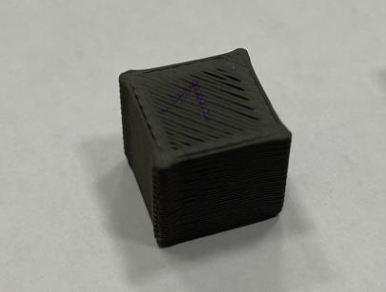
\includegraphics[width=0.5\linewidth]{bilder/Testdruck auf Raise Pro 3D.png}
        \caption[Testdruck von dem Raise3D Pro2 Plus - Isometrische Ansicht] {Testdruck von dem Raise3D Pro2 Plus - Isometrische Ansicht (Eigene Darstellung)}
	\label{erster Druck - Isometrie}
\end{figure}
\begin{figure}[h]
	\centering
	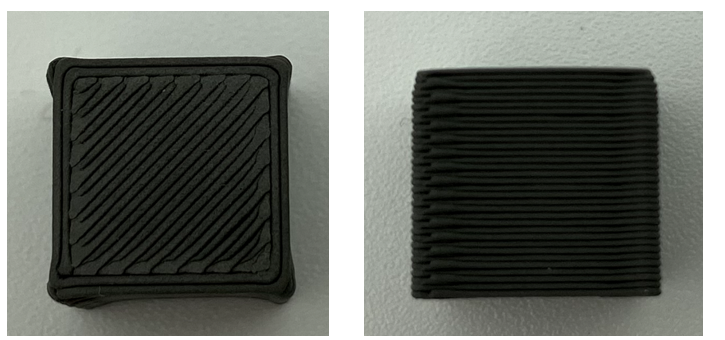
\includegraphics[width=\linewidth]{bilder/Testdruck auf Raise Pro 3D Seitenansicht - Draufsicht.png}
        \caption[Erster Testdruck mit dem Raise3D Pro2 Plus - Seitenansicht und Draufsicht] {Erster Testdruck mit dem Raise3D Pro2 Plus -Draufsicht (l) und Seitenansicht (r) (Geschwindigkeit: 60mm/s; Schichthöhe: 0,4mm) (Eigene Darstellung)}
	\label{erster Druck - Seitenansicht}
\end{figure}

Erkennbar ist hier deutlich, die Ungenauigkeit des Drucks dargestellt. Dies lässt sich sehr gut in \autoref{erster Druck - Seitenansicht} an den Ecken in der rechten Draufsicht erkennen. Das Symptom der zu stark abgerundeten Ecken ist auf das Fehlen von linearer Vorschubtechnik aus \autoref{sec:LineareVorschub} zurückzuführen. Die Extrusionsrate ist nicht an das Be- und Entschleunigungsverhalten des Druckkopfs angepasst. Dadurch ist an den Ecken, in denen die Geschwindigkeit langsamer ist, mehr Material aufgetragen. Die Einstellung der linearen Vorschubregelung lässt sich bei diesem Drucker nicht einstellen und die \textit{Firmware} ist nicht \textit{Open Source}. Deshalb ist es schwierig ohne zusätzliche Hardware diese Funktion nachträglich zu implementieren.

Bei Verringerung der Geschwindigkeit von 60mm/s auf 20mm/s ist dieser Effekt deutlich verringert. In \autoref{zweiter Druck - Isometrie} ist das Ergebnis der Verringerung der Geschwindigkeit und der Schichthöhe dargestellt. Doch diese Optimierung geht zu Lasten der gesamten Druckzeit. 

\begin{figure}[h]
	\centering
	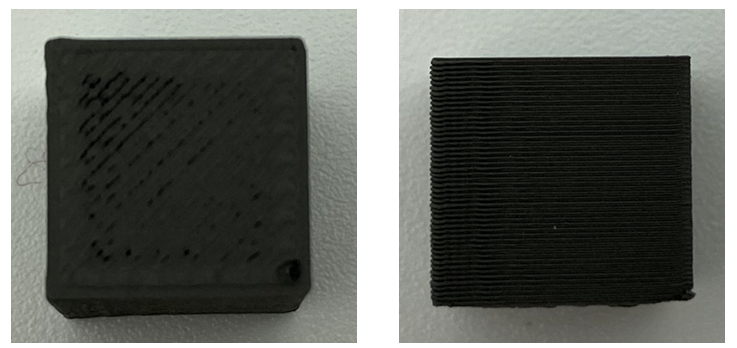
\includegraphics[width=\linewidth]{bilder/2. Testdruck auf Raise Pro 3D Seitenansicht - Draufsicht.png}
        \caption[Zweiter Testdruck mit dem Raise3D Pro2 Plus - Isometrische Ansicht] {Zweiter Testdruck mit dem Raise3D Pro2 Plus -Draufsicht (l) und Seitenansicht (r) (Geschwindigkeit: 20mm/s; Schichthöhe: 0,1mm) (Eigene Darstellung)}
	\label{zweiter Druck - Isometrie}
\end{figure}

\section{Verwendung des Prusa i3 MK3S+}
\label{Drucker}

Mit dem \textit{Raise 3D Pro 2} sind die Ergebnisse aufgrund der fehlenden Einstellmöglichkeit der linearen Vorschubregelung (siehe \autoref{sec:LineareVorschub}) nicht zufriedenstellend. Da auch die verlängerte Druckzeit bei verringerter Geschwindigkeit nicht negativ zu bewerten ist, wird in dieser Arbeit auf den \textit{i3 MK3S+} der Firma \textit{Prusa} zurückgegriffen. Dieser hat ebenfalls wie der \textit{Raise3D}-Drucker einen Druckkopf mit Direktextruder (siehe \autoref{sec:ArtenFDM}). Dies ist vom Filamenthersteller aufgrund des spröden Materials empfohlen.

\begin{figure}[h]
	\centering
	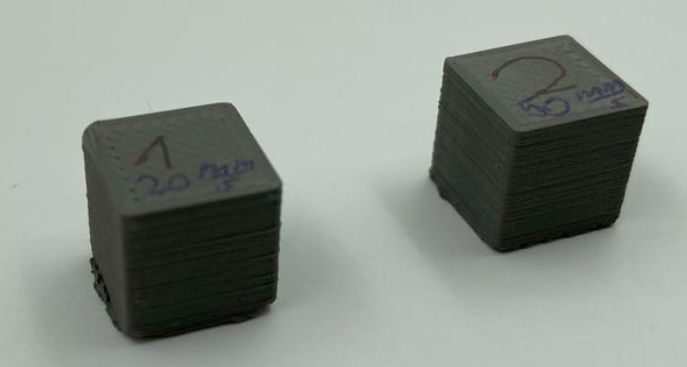
\includegraphics[width=\linewidth]{bilder/Erster Testdruck mit Prusa.png}
        \caption[Erster (20mm/s) und zweiter (50mm/s) Testdruck mit dem Prusa]{Erster (20mm/s) und zweiter (50mm/s) Testdruck mit dem Prusa (Eigene Darstellung)}
	\label{Erster Testdruck Prusa}
\end{figure}

Der erste Testdruck mit dem \textit{Prusa} ist in \autoref{Erster Testdruck Prusa} links dargestellt. Die Einstellungen gleichen den Einstellungen aus \autocite{M.Mickan}
(siehe \autoref{ursprüngliche Werte}). Die Geschwindigkeit ist jedoch auf 20mm/s reduziert und die Schichthöhe beträgt 0,1mm. Aufgrund des fehlerfreien Ergebnisses wird ebenso ein Würfel mit einer Druckgeschwindigkeit von 50mm/s gedruckt. Dieser ist in \autoref{Erster Testdruck Prusa} rechts dargestellt. Somit stehen die Parameter für die Würfel und die liegenden Zugproben fest. Sie sind in \autoref{Würfelparameter} aufgefasst. 

\section{Probenherstellung und -messung}

Die Testwürfel und die Zugproben sind in dem CAD-System \textit{NX12} erstellt. Die erzeugten Würfel haben eine Kantenlänge von 10mm. Diese sind dann als STL-Datei exportiert und mit \textit{Ultimaker Cura Version 5.3.1} mit den Einstellungen nach \autoref{Würfelparameter} geslict, also ein \textit{g-code} wurde abgeleitet. Wie bereits erwähnt wird für den Druck der \textit{Prusa MK3S+} mit einer verwendet. Auf dem originalen Druckbetts des \textit{Prusa} wird eine Schicht aus Flachkreppband der Marke \textit{Günter Seits} geklebt. Ohne dieses Flachkreppband haftet die erste Schicht zu gut an dem Druckbett, dadurch ist es unmöglich das Bauteil zerstörungsfrei von dem Druckbett zu lösen.\\
Die Würfel werden nun als Grünteil mit einem Digitalmessschieber der Marke \textit{Mitutoyo} gemessen. Die Proben werden einzeln mit einer \textit{Kern PRS 620-3} gewogen. Die Messwerte, samt errechnetem Volumen und Dichte sind in \autoref{Grünteilmaße} aufgeführt.